\section{Результаты работы программы}

При запуске программа выводит консольное меню (рис.~\ref{fig:menu}),
разбитое на пять разделов по лабораторным работам.
Перед запуском любого алгоритма необходимо сгенерировать граф (пункт~1),
выбрав число вершин, тип ориентированности и знак весов.

\begin{figure}[H]
    \centering
    
\includegraphics[width=0.6\linewidth]{photo/screen/menu.jpg}
    \caption{Главное меню программы}
    \label{fig:menu}
\end{figure}

\subsection{Генерация графа (пункты~1--3)}

Пункт~1 запрашивает число вершин, тип ориентированности и знак весов,
после чего генерирует граф по распределению Вейбулла.
На рис.~\ref{fig:gen_or} и~\ref{fig:gen_neor} показаны примеры генерации
ориентированного и неориентированного графов.
Пункты~2 и~3 выводят матрицы смежности и весов
(рис.~\ref{fig:or_s}--\ref{fig:neor_w}).

\begin{figure}[H]
    \centering
    \begin{minipage}[t]{0.48\linewidth}
        \vspace{0pt}
        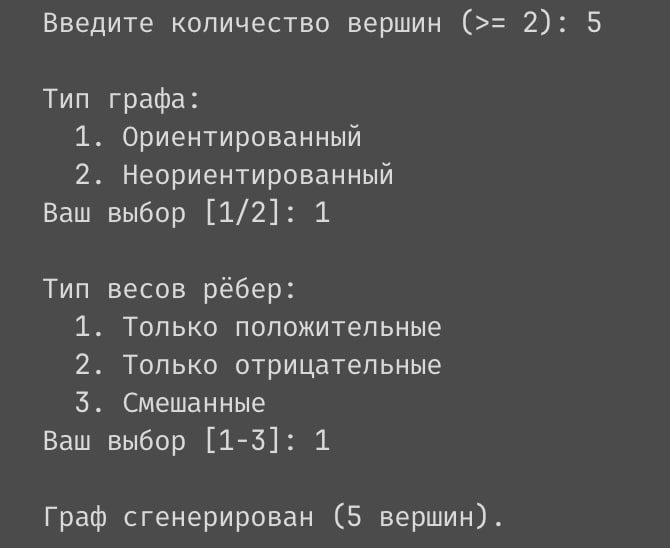
\includegraphics[width=\linewidth]{photo/screen/gen_or.jpg}
        \caption{Генерация ориентированного графа (пункт~1)}
        \label{fig:gen_or}
    \end{minipage}\hfill
    \begin{minipage}[t]{0.48\linewidth}
        \vspace{0pt}
        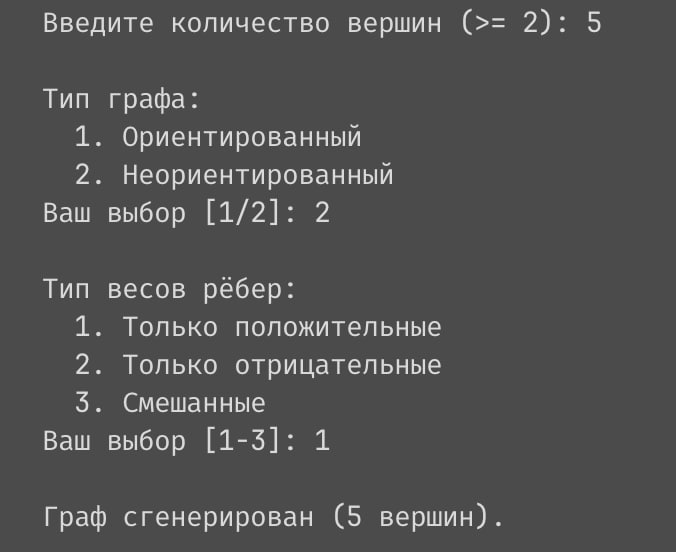
\includegraphics[width=\linewidth]{photo/screen/gen_neor.jpg}
        \caption{Генерация неориентированного графа (пункт~1)}
        \label{fig:gen_neor}
    \end{minipage}
\end{figure}

\begin{figure}[H]
    \centering
    \begin{minipage}[t]{0.48\linewidth}
        \vspace{0pt}
        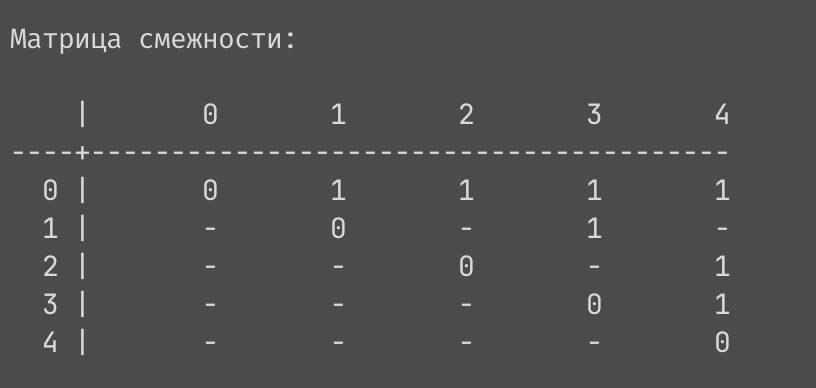
\includegraphics[width=\linewidth]{photo/screen/or_s.jpg}
        \caption{Матрица смежности ориентированного графа (пункт~2)}
        \label{fig:or_s}
    \end{minipage}\hfill
    \begin{minipage}[t]{0.48\linewidth}
        \vspace{0pt}
        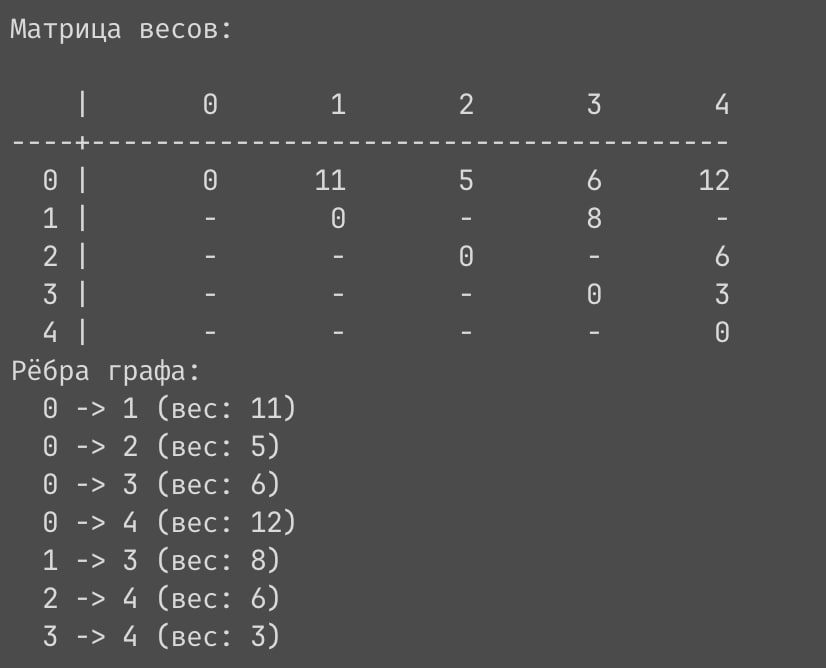
\includegraphics[width=\linewidth]{photo/screen/or_w.jpg}
        \caption{Матрица весов ориентированного графа (пункт~3)}
        \label{fig:or_w}
    \end{minipage}
\end{figure}

\begin{figure}[H]
    \centering
    \begin{minipage}[t]{0.48\linewidth}
        \vspace{0pt}
        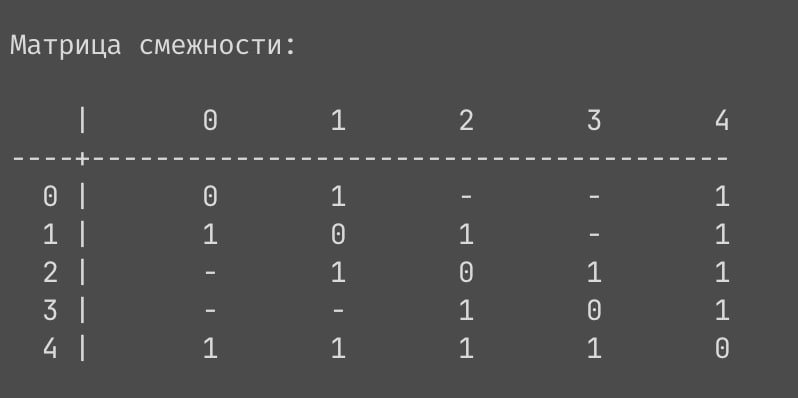
\includegraphics[width=\linewidth]{photo/screen/neor_s.jpg}
        \caption{Матрица смежности неориентированного графа (пункт~2)}
        \label{fig:neor_s}
    \end{minipage}\hfill
    \begin{minipage}[t]{0.48\linewidth}
        \vspace{0pt}
        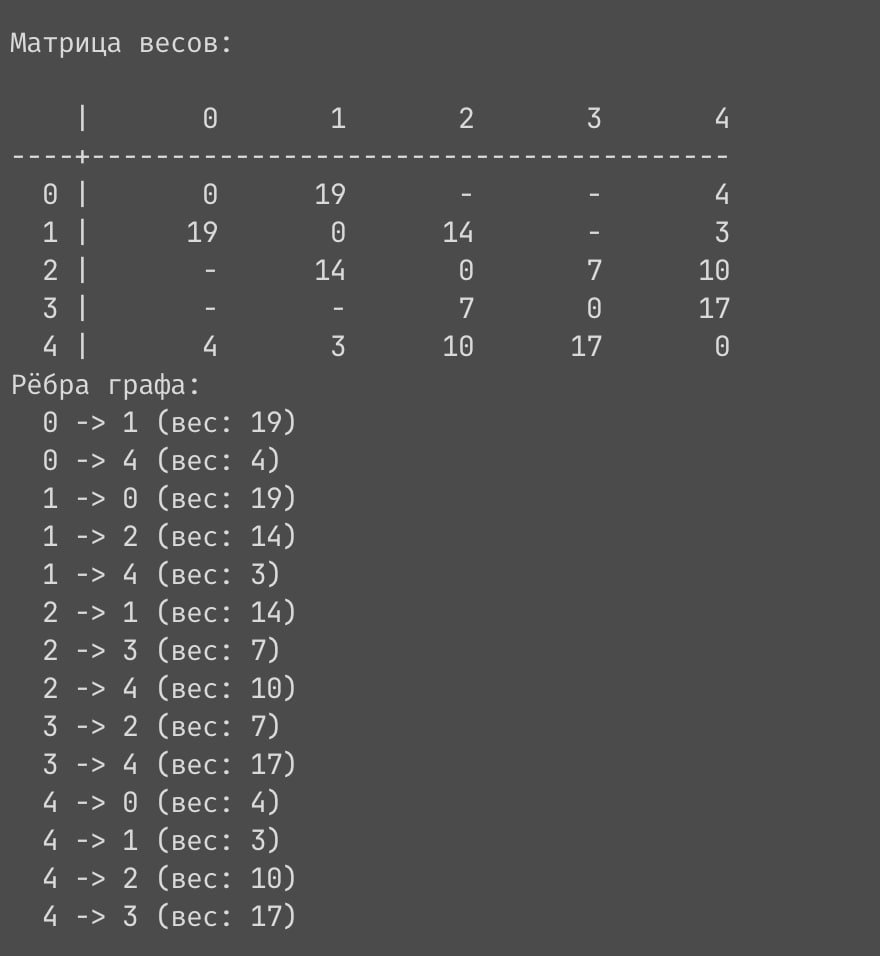
\includegraphics[width=\linewidth]{photo/screen/neor_w.jpg}
        \caption{Матрица весов неориентированного графа (пункт~3)}
        \label{fig:neor_w}
    \end{minipage}
\end{figure}

\subsection{Лабораторная работа~1 (пункты~4--8)}

В первой лабораторной работе вычисляются метрики графа и ищутся пути.
Пункт~4 (рис.~\ref{fig:p4}) выводит эксцентриситет каждой вершины.
Пункт~5 (рис.~\ref{fig:p5}) находит центр графа и его радиус.
Пункт~6 (рис.~\ref{fig:p6}) выводит диаметр и диаметральные вершины
вместе с путями между ними.
Пункт~7 (рис.~\ref{fig:p7min},~\ref{fig:p7max}) строит матрицу Шимбелла
для минимальных и максимальных путей заданной длины $k$.
Пункт~8 (рис.~\ref{fig:p8}) перечисляет все простые пути между двумя
заданными вершинами.

\begin{figure}[H]
    \centering
    \begin{minipage}[t]{0.48\linewidth}
        \vspace{0pt}
        
\includegraphics[width=\linewidth]{photo/screen/4.jpg}
        \caption{Пункт~4: эксцентриситеты вершин}
        \label{fig:p4}
    \end{minipage}\hfill
    \begin{minipage}[t]{0.48\linewidth}
        \vspace{0pt}
        
\includegraphics[width=\linewidth]{photo/screen/5.jpg}
        \caption{Пункт~5: центр графа и радиус}
        \label{fig:p5}
    \end{minipage}
\end{figure}

\begin{figure}[H]
    \centering
    
\includegraphics[width=0.75\linewidth]{photo/screen/6.jpg}
    \caption{Пункт~6: диаметр графа и диаметральные вершины с путями}
    \label{fig:p6}
\end{figure}

\begin{figure}[H]
    \centering
    \begin{minipage}[t]{0.48\linewidth}
        \vspace{0pt}
        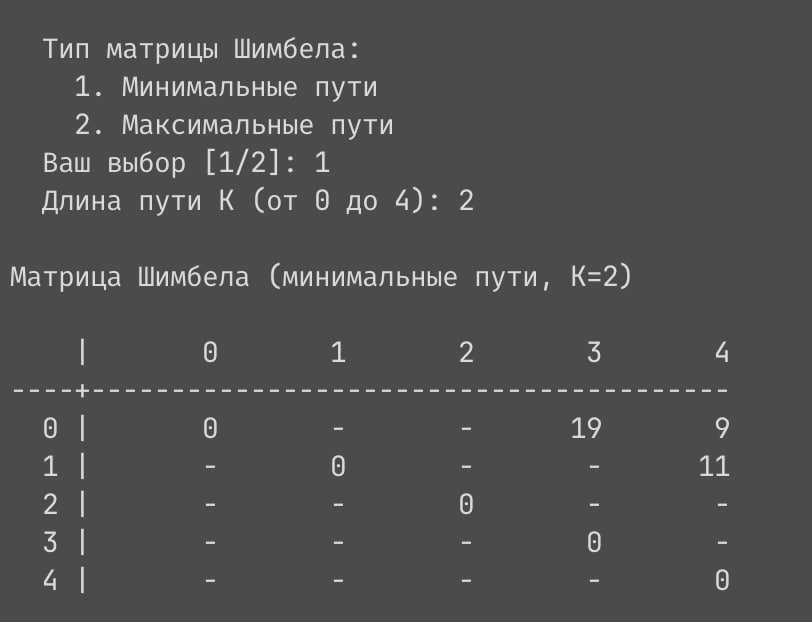
\includegraphics[width=\linewidth]{photo/screen/7_min.jpg}
        \caption{Пункт~7: матрица Шимбелла -- минимальные пути}
        \label{fig:p7min}
    \end{minipage}\hfill
    \begin{minipage}[t]{0.48\linewidth}
        \vspace{0pt}
        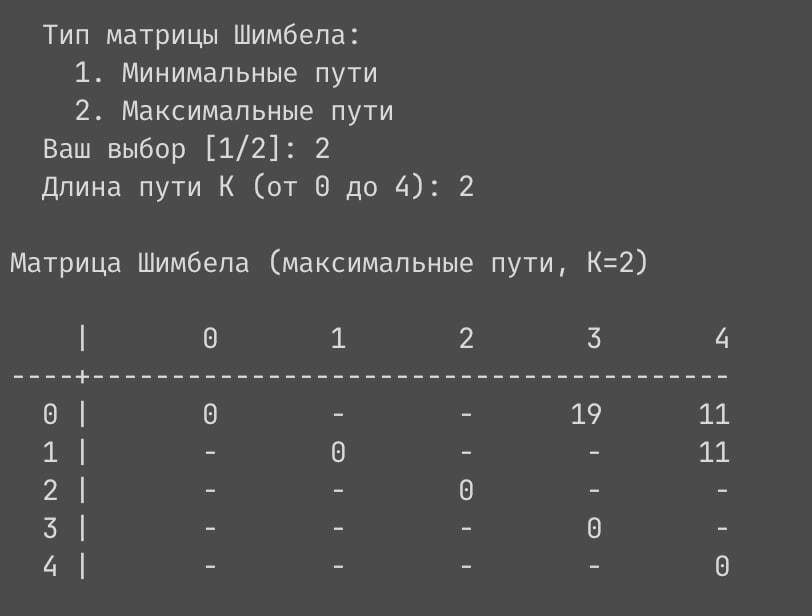
\includegraphics[width=\linewidth]{photo/screen/7_max.jpg}
        \caption{Пункт~7: матрица Шимбелла -- максимальные пути}
        \label{fig:p7max}
    \end{minipage}
\end{figure}

\begin{figure}[H]
    \centering
    
\includegraphics[width=0.75\linewidth]{photo/screen/8.jpg}
    \caption{Пункт~8: все простые пути от вершины $A$ до вершины $B$}
    \label{fig:p8}
\end{figure}

\subsection{Лабораторная работа~2 (пункты~9--11)}

Во второй лабораторной работе реализованы топологическая сортировка
и поиск кратчайших путей.
Пункт~9 (рис.~\ref{fig:p9}) выполняет топологическую сортировку
алгоритмом Фалкерсона и выводит перенумерованные матрицы.
Пункт~10 (рис.~\ref{fig:p10}) вычисляет матрицу расстояний
алгоритмом Флойда-Уоршалла и выводит кратчайший путь между двумя вершинами.
Пункт~11 (рис.~\ref{fig:p11}) сравнивает оба алгоритма по числу итераций.

\begin{figure}[H]
    \centering
    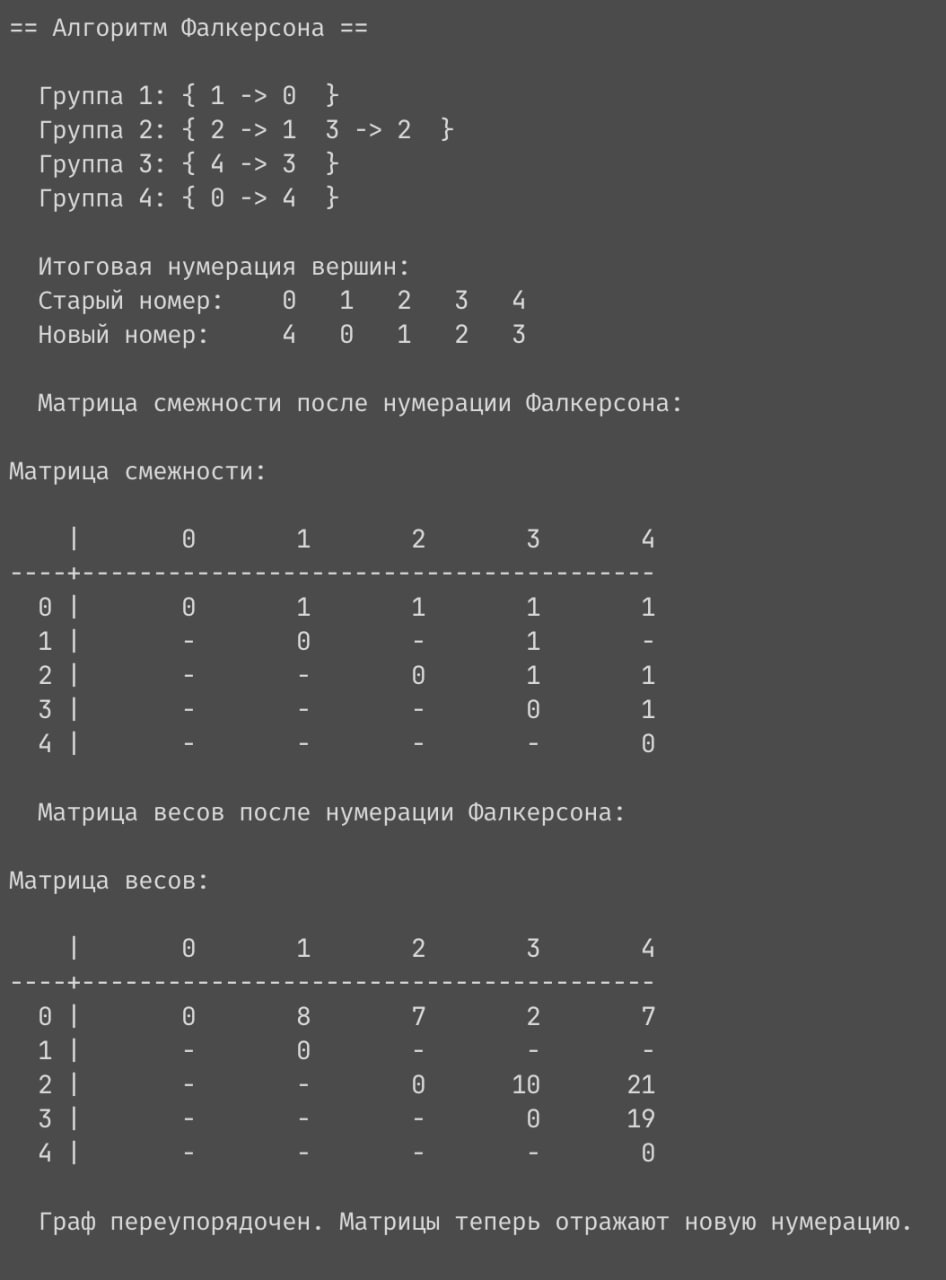
\includegraphics[width=0.75\linewidth]{photo/screen/9.jpg}
    \caption{Пункт~9: топологическая сортировка алгоритмом Фалкерсона}
    \label{fig:p9}
\end{figure}

\begin{figure}[H]
    \centering
    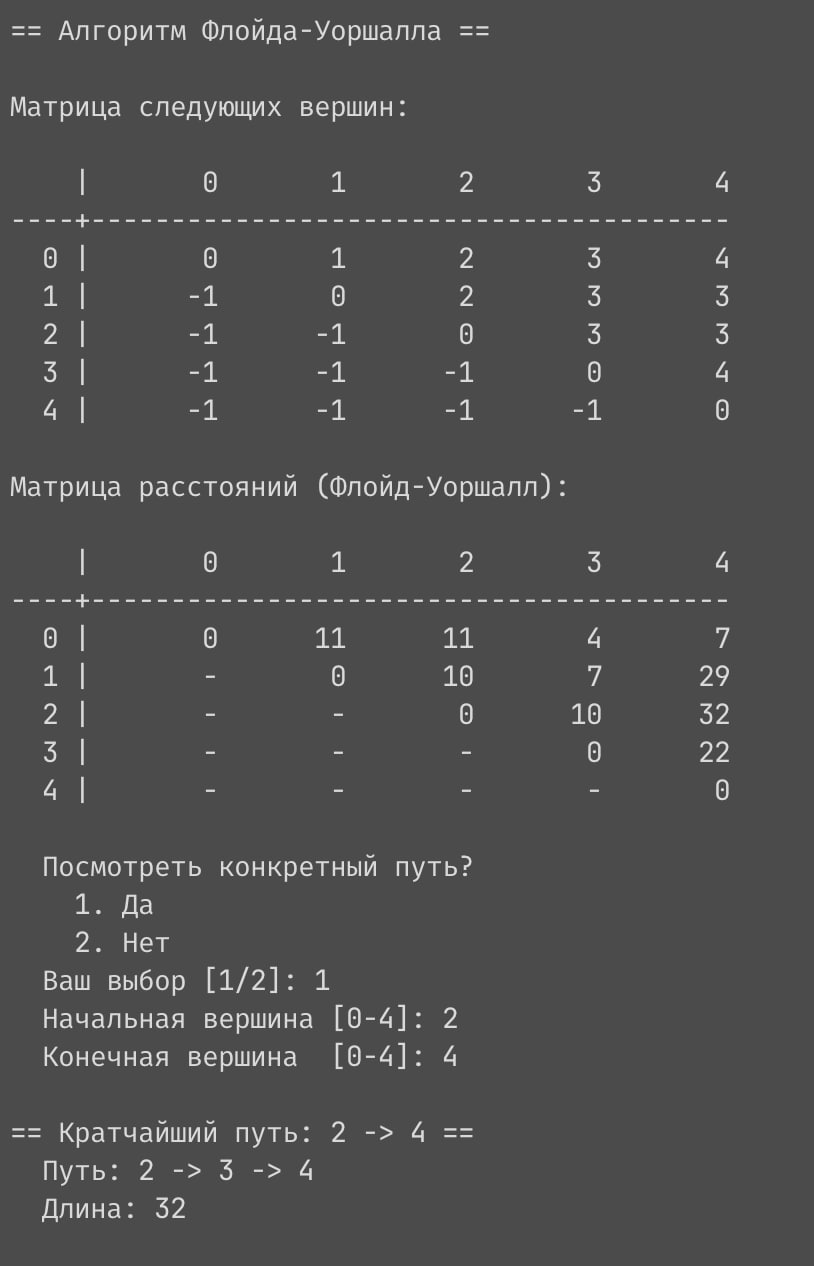
\includegraphics[width=0.75\linewidth]{photo/screen/10.jpg}
    \caption{Пункт~10: матрица расстояний и кратчайший путь (Флойд-Уоршалл)}
    \label{fig:p10}
\end{figure}

\begin{figure}[H]
    \centering
    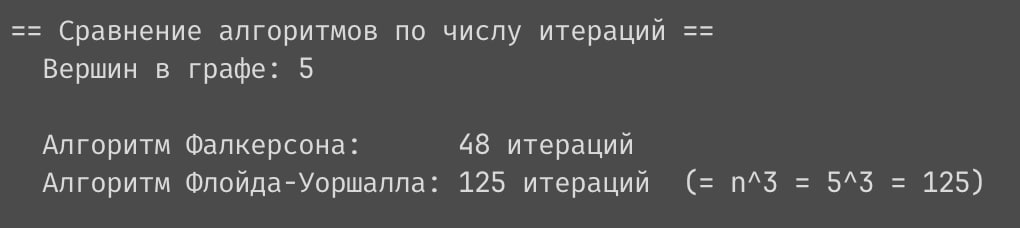
\includegraphics[width=0.75\linewidth]{photo/screen/11.jpg}
    \caption{Пункт~11: сравнение числа итераций алгоритмов Фалкерсона и Флойда-Уоршалла}
    \label{fig:p11}
\end{figure}

\subsection{Лабораторная работа~3 (пункты~12--15)}

В третьей лабораторной работе реализована транспортная сеть с поиском
максимального потока и потока минимальной стоимости.
Пункты~12 и~13 (рис.~\ref{fig:p12},~\ref{fig:p13}) выводят матрицы
пропускных способностей и стоимостей.
Пункт~14 (рис.~\ref{fig:p14}) находит максимальный поток алгоритмом
Эдмондса--Карпа.
Пункт~15 (рис.~\ref{fig:p15_1}--\ref{fig:p15_3}) вычисляет поток
минимальной стоимости величиной $\lfloor 2/3 \cdot F_{\max} \rfloor$.

\begin{figure}[H]
    \centering
    \begin{minipage}[t]{0.48\linewidth}
        \vspace{0pt}
        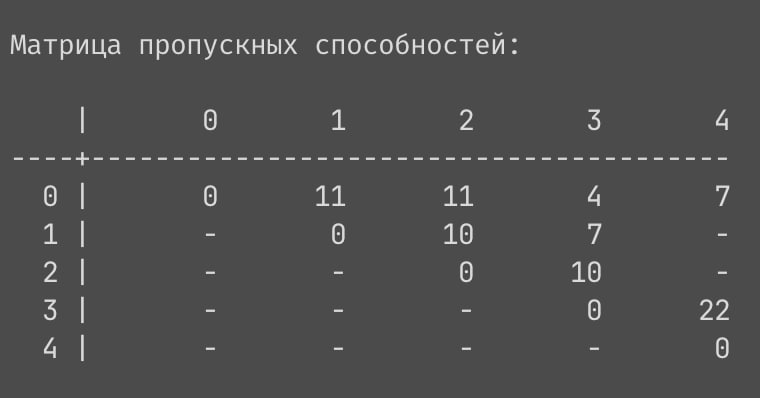
\includegraphics[width=\linewidth]{photo/screen/12.jpg}
        \caption{Пункт~12: матрица пропускных способностей}
        \label{fig:p12}
    \end{minipage}\hfill
    \begin{minipage}[t]{0.48\linewidth}
        \vspace{0pt}
        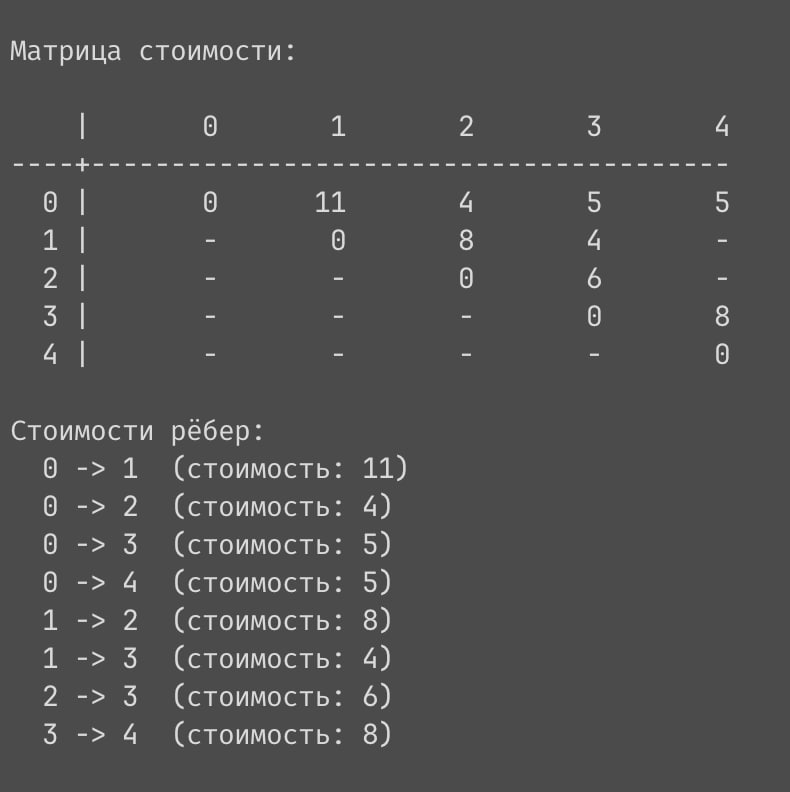
\includegraphics[width=\linewidth]{photo/screen/13.jpg}
        \caption{Пункт~13: матрица стоимостей рёбер}
        \label{fig:p13}
    \end{minipage}
\end{figure}

\begin{figure}[H]
    \centering
    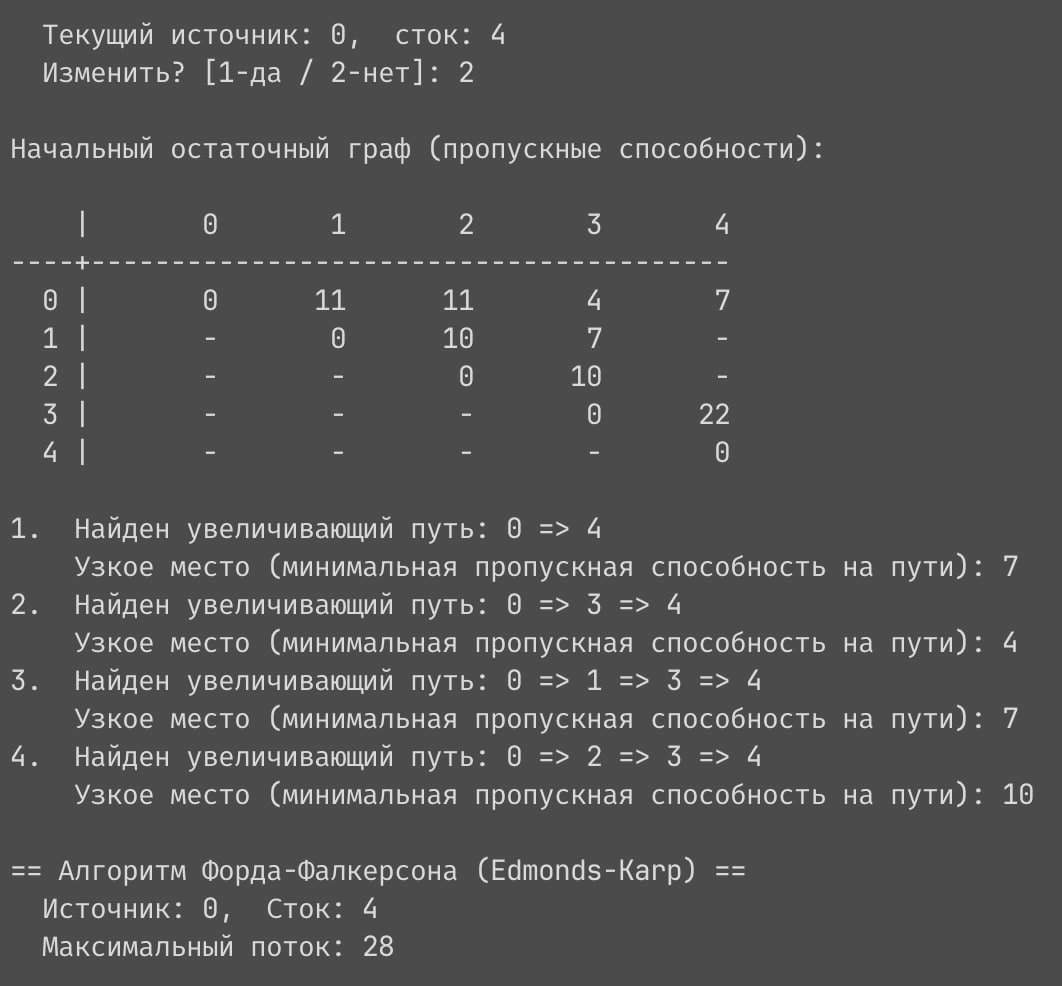
\includegraphics[width=0.75\linewidth]{photo/screen/14.jpg}
    \caption{Пункт~14: максимальный поток алгоритмом Эдмондса--Карпа}
    \label{fig:p14}
\end{figure}

\begin{figure}[H]
    \centering
    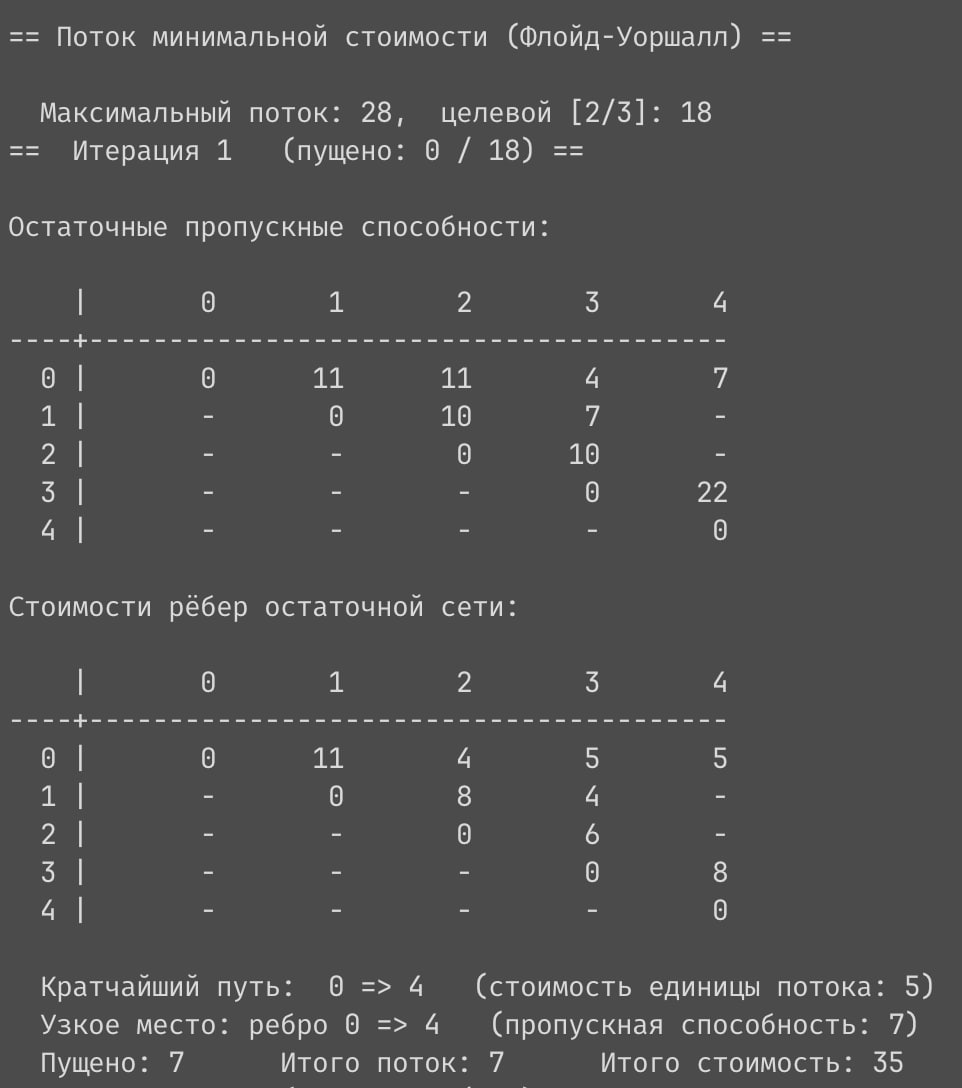
\includegraphics[width=0.75\linewidth]{photo/screen/15_1.jpg}
    \caption{Пункт~15: итерации поиска потока минимальной стоимости}
    \label{fig:p15_1}
\end{figure}

\begin{figure}[H]
    \centering
    \begin{minipage}[t]{0.48\linewidth}
        \vspace{0pt}
        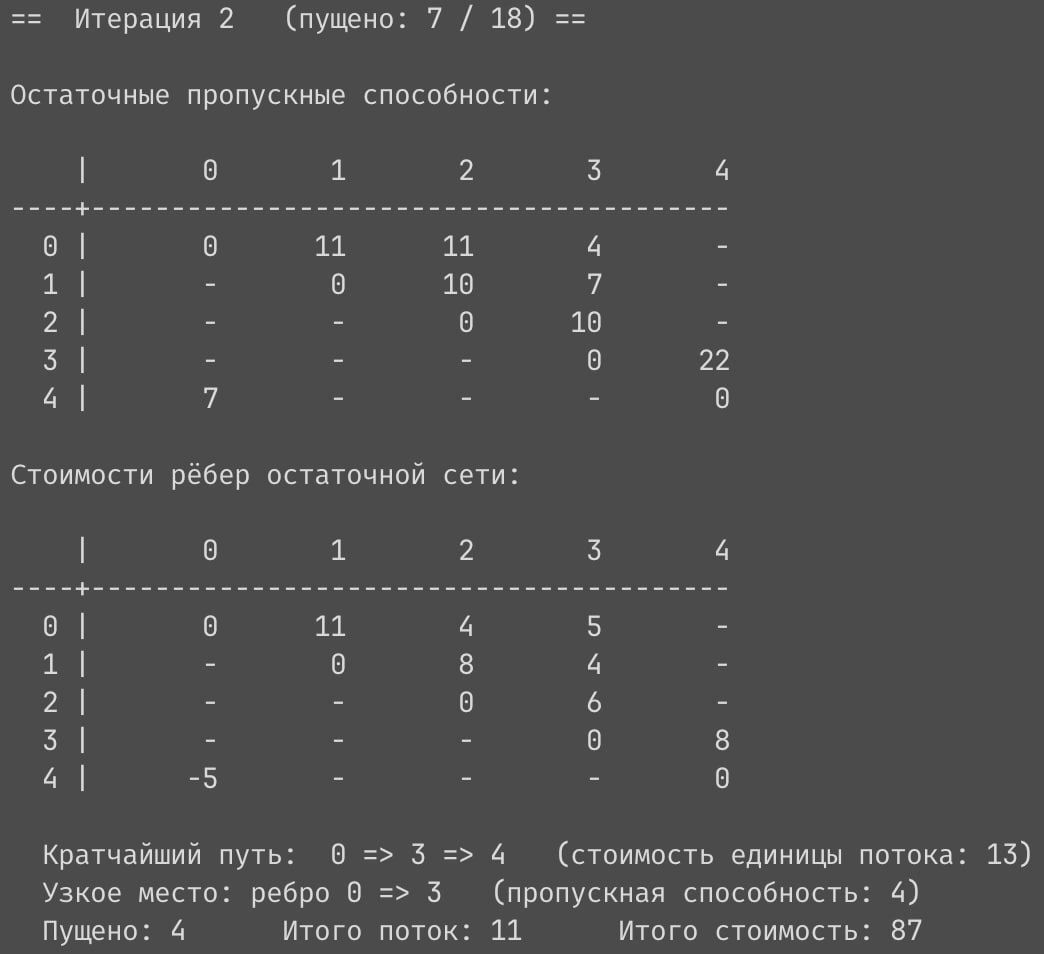
\includegraphics[width=\linewidth]{photo/screen/15_2.jpg}
        \caption{Пункт~15: продолжение итераций}
        \label{fig:p15_2}
    \end{minipage}\hfill
    \begin{minipage}[t]{0.48\linewidth}
        \vspace{0pt}
        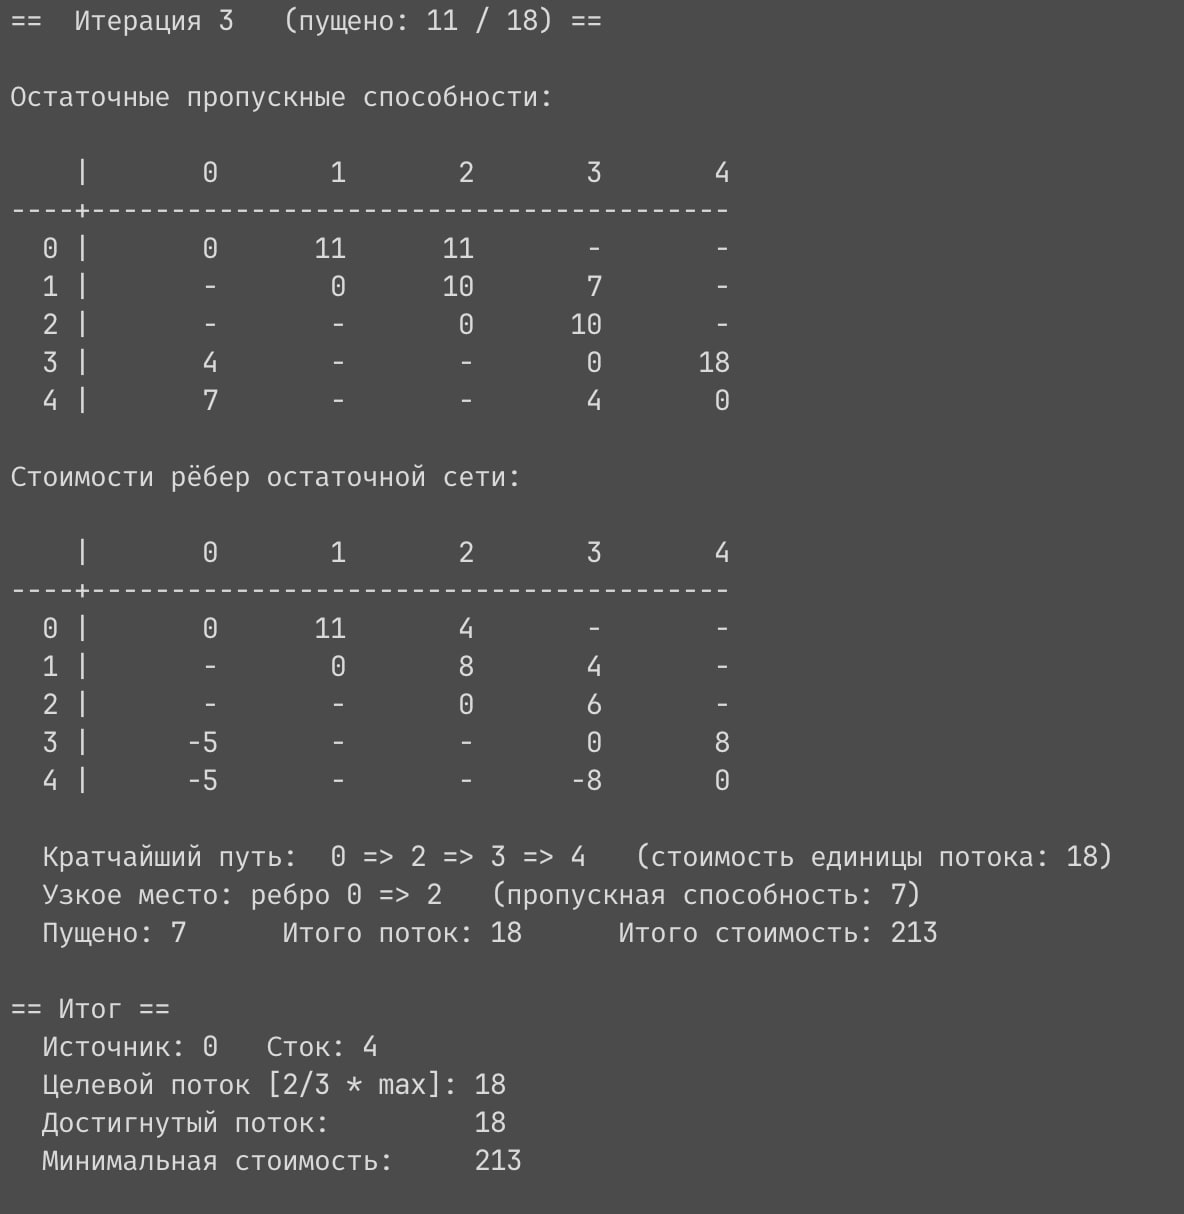
\includegraphics[width=\linewidth]{photo/screen/15_3.jpg}
        \caption{Пункт~15: итоговый поток и минимальная стоимость}
        \label{fig:p15_3}
    \end{minipage}
\end{figure}

\subsection{Лабораторная работа~4 (пункты~16--20)}

В четвёртой лабораторной работе выполняются операции с остовными деревьями
и независимыми множествами.
Пункт~16 (рис.~\ref{fig:p16}) считает число остовных деревьев
по теореме Кирхгофа.
Пункт~17 (рис.~\ref{fig:p17}) строит минимальный остов алгоритмом Краскала.
Пункты~18 и~19 (рис.~\ref{fig:p18},~\ref{fig:p19}) кодируют остов
кодом Прюфера и декодируют его обратно с сохранением весов.
Пункт~20 (рис.~\ref{fig:p20_1},~\ref{fig:p20_2}) ищет максимальное
независимое множество на исходном графе и на остове.

\begin{figure}[H]
    \centering
    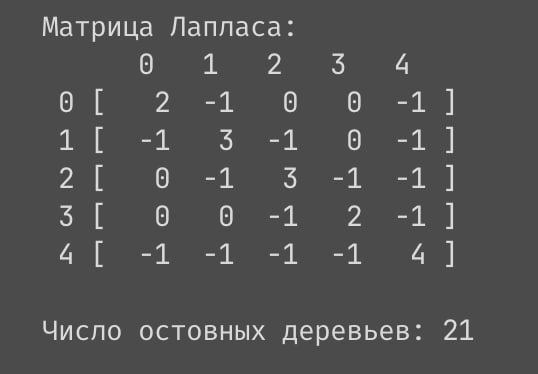
\includegraphics[width=0.75\linewidth]{photo/screen/16.jpg}
    \caption{Пункт~16: матрица Лапласа и число остовных деревьев (теорема Кирхгофа)}
    \label{fig:p16}
\end{figure}

\begin{figure}[H]
    \centering
    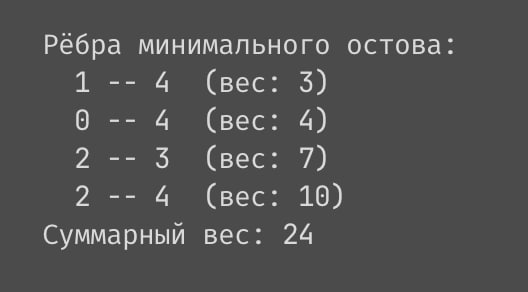
\includegraphics[width=0.75\linewidth]{photo/screen/17.jpg}
    \caption{Пункт~17: минимальный остов алгоритмом Краскала}
    \label{fig:p17}
\end{figure}

\begin{figure}[H]
    \centering
    \begin{minipage}[t]{0.48\linewidth}
        \vspace{0pt}
        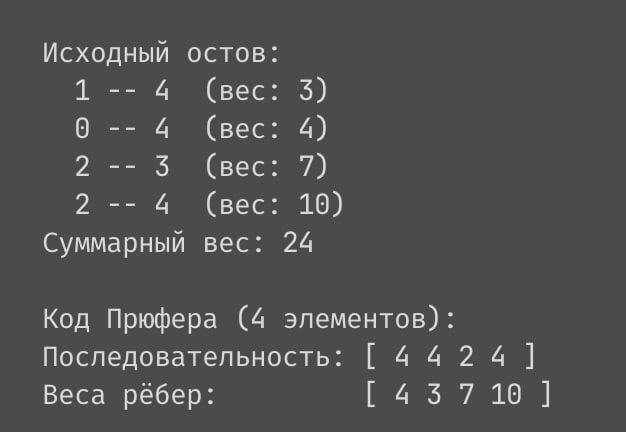
\includegraphics[width=\linewidth]{photo/screen/18.jpg}
        \caption{Пункт~18: кодирование остова кодом Прюфера}
        \label{fig:p18}
    \end{minipage}\hfill
    \begin{minipage}[t]{0.48\linewidth}
        \vspace{0pt}
        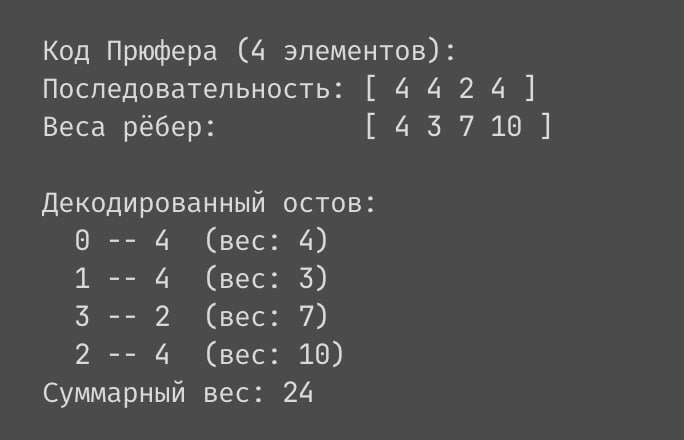
\includegraphics[width=\linewidth]{photo/screen/19.jpg}
        \caption{Пункт~19: декодирование кода Прюфера}
        \label{fig:p19}
    \end{minipage}
\end{figure}

\begin{figure}[H]
    \centering
    \begin{minipage}[t]{0.48\linewidth}
        \vspace{0pt}
        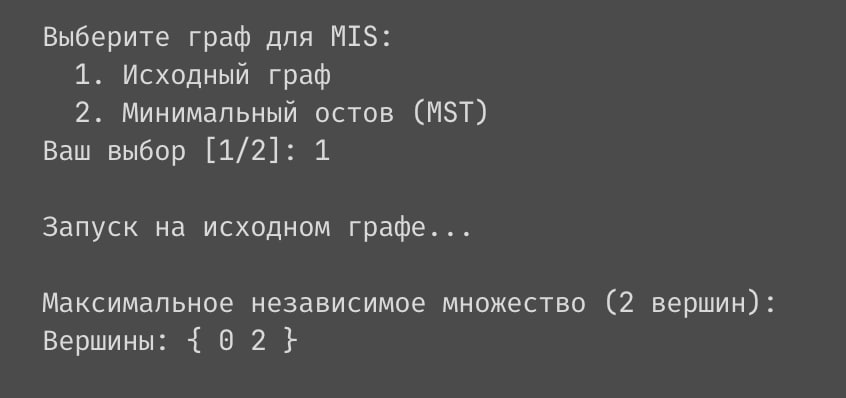
\includegraphics[width=\linewidth]{photo/screen/20_1.jpg}
        \caption{Пункт~20: МНМ на исходном графе}
        \label{fig:p20_1}
    \end{minipage}\hfill
    \begin{minipage}[t]{0.48\linewidth}
        \vspace{0pt}
        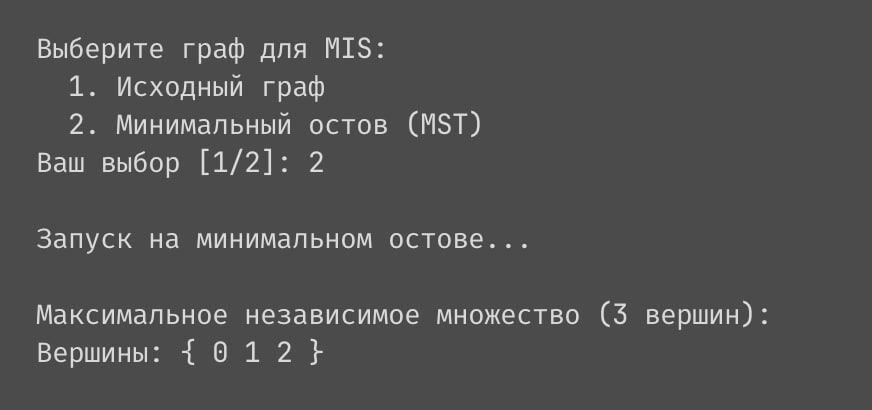
\includegraphics[width=\linewidth]{photo/screen/20_2.jpg}
        \caption{Пункт~20: МНМ на минимальном остове}
        \label{fig:p20_2}
    \end{minipage}
\end{figure}

\subsection{Лабораторная работа~5 (пункты~21--23)}

В пятой лабораторной работе реализованы эйлеровы графы и система циклов.
Пункт~21 (рис.~\ref{fig:p21}) проверяет эйлеровость графа, при необходимости
достраивает его и строит эйлеров цикл алгоритмом Хирхольцера.
Пункт~22 (рис.~\ref{fig:p22}) вычисляет фундаментальную систему циклов
на основе минимального остова.
Пункт~23 (рис.~\ref{fig:p23}) вычисляет симметрическую разность
выбранных фундаментальных циклов.

\begin{figure}[H]
    \centering
    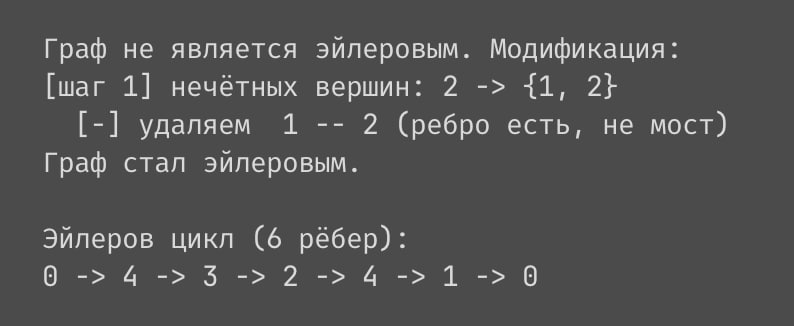
\includegraphics[width=0.75\linewidth]{photo/screen/21.jpg}
    \caption{Пункт~21: достройка до эйлерового графа и построение эйлерова цикла}
    \label{fig:p21}
\end{figure}

\begin{figure}[H]
    \centering
    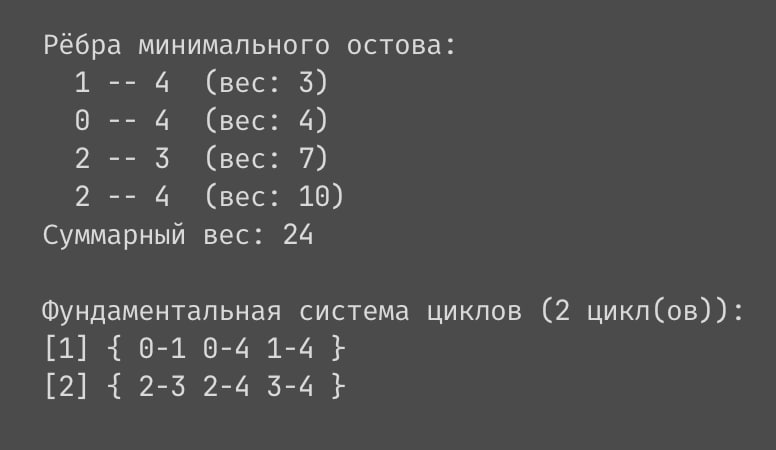
\includegraphics[width=0.75\linewidth]{photo/screen/22.jpg}
    \caption{Пункт~22: фундаментальная система циклов на основе МОД}
    \label{fig:p22}
\end{figure}

\begin{figure}[H]
    \centering
    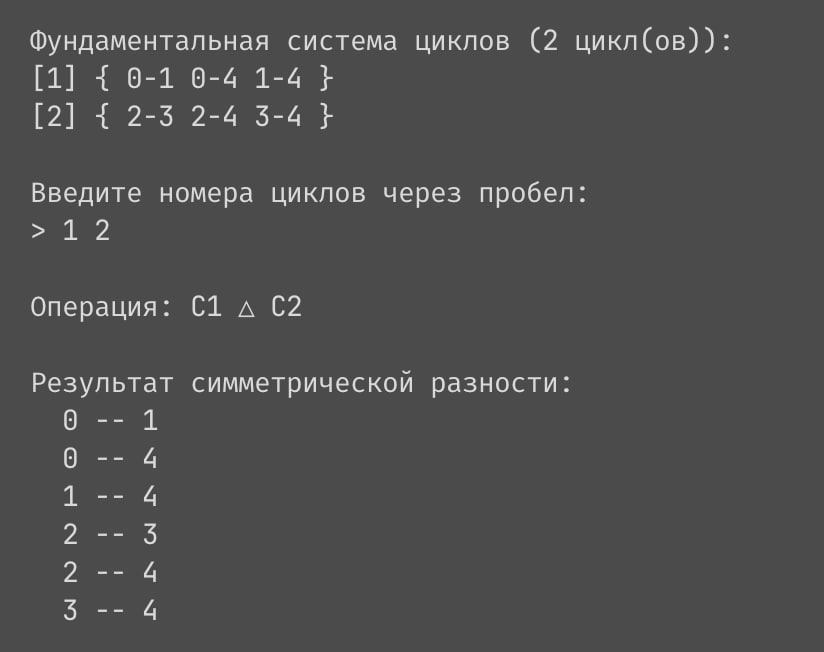
\includegraphics[width=0.75\linewidth]{photo/screen/23.jpg}
    \caption{Пункт~23: симметрическая разность фундаментальных циклов}
    \label{fig:p23}
\end{figure}
